\documentclass[11pt, a4paper]{article}
\usepackage{amsmath}
\usepackage{listings}
\usepackage{xcolor}
\usepackage{graphicx} % Required for including images
\usepackage{color} % Required for custom colors
\usepackage{makeidx}
\usepackage{caption}

\captionsetup[figure]{justification=centering}

\makeindex

\usepackage{hyperref} % Add hyperlinks to references

% Define custom colors
\definecolor{codegreen}{rgb}{0,0.6,0}
\definecolor{codegray}{rgb}{0.5,0.5,0.5}
\definecolor{codepurple}{rgb}{0.58,0,0.82}
\definecolor{backcolour}{rgb}{0.95,0.95,0.92}

\lstset{
  basicstyle=\tiny\ttfamily, % Adjust the font size here
  language=Python,
  frame=single,
  breaklines=true,
  postbreak=\mbox{$\hookrightarrow$},
  showstringspaces=false,
  numbers=left,
  captionpos=b,
  keywordstyle=\color{magenta},      % Style for keywords
  commentstyle=\color{codegreen},    % Style for comments
  stringstyle=\color{codepurple},    % Style for strings
  numberstyle=\tiny\color{codegray}, % Style for line numbers
  rulecolor=\color{black},           % Frame color
  backgroundcolor=\color{backcolour}% Background color
}


\title{Optimal Path Analysis: Beach Scenarios}
\author{ChatGPT (gpt v4) [90\%] \& Peter Sels [9\%] \& Don Frodo [1\%]}
\date{}


\begin{document}

\maketitle


\begin{figure}[h]
\centering
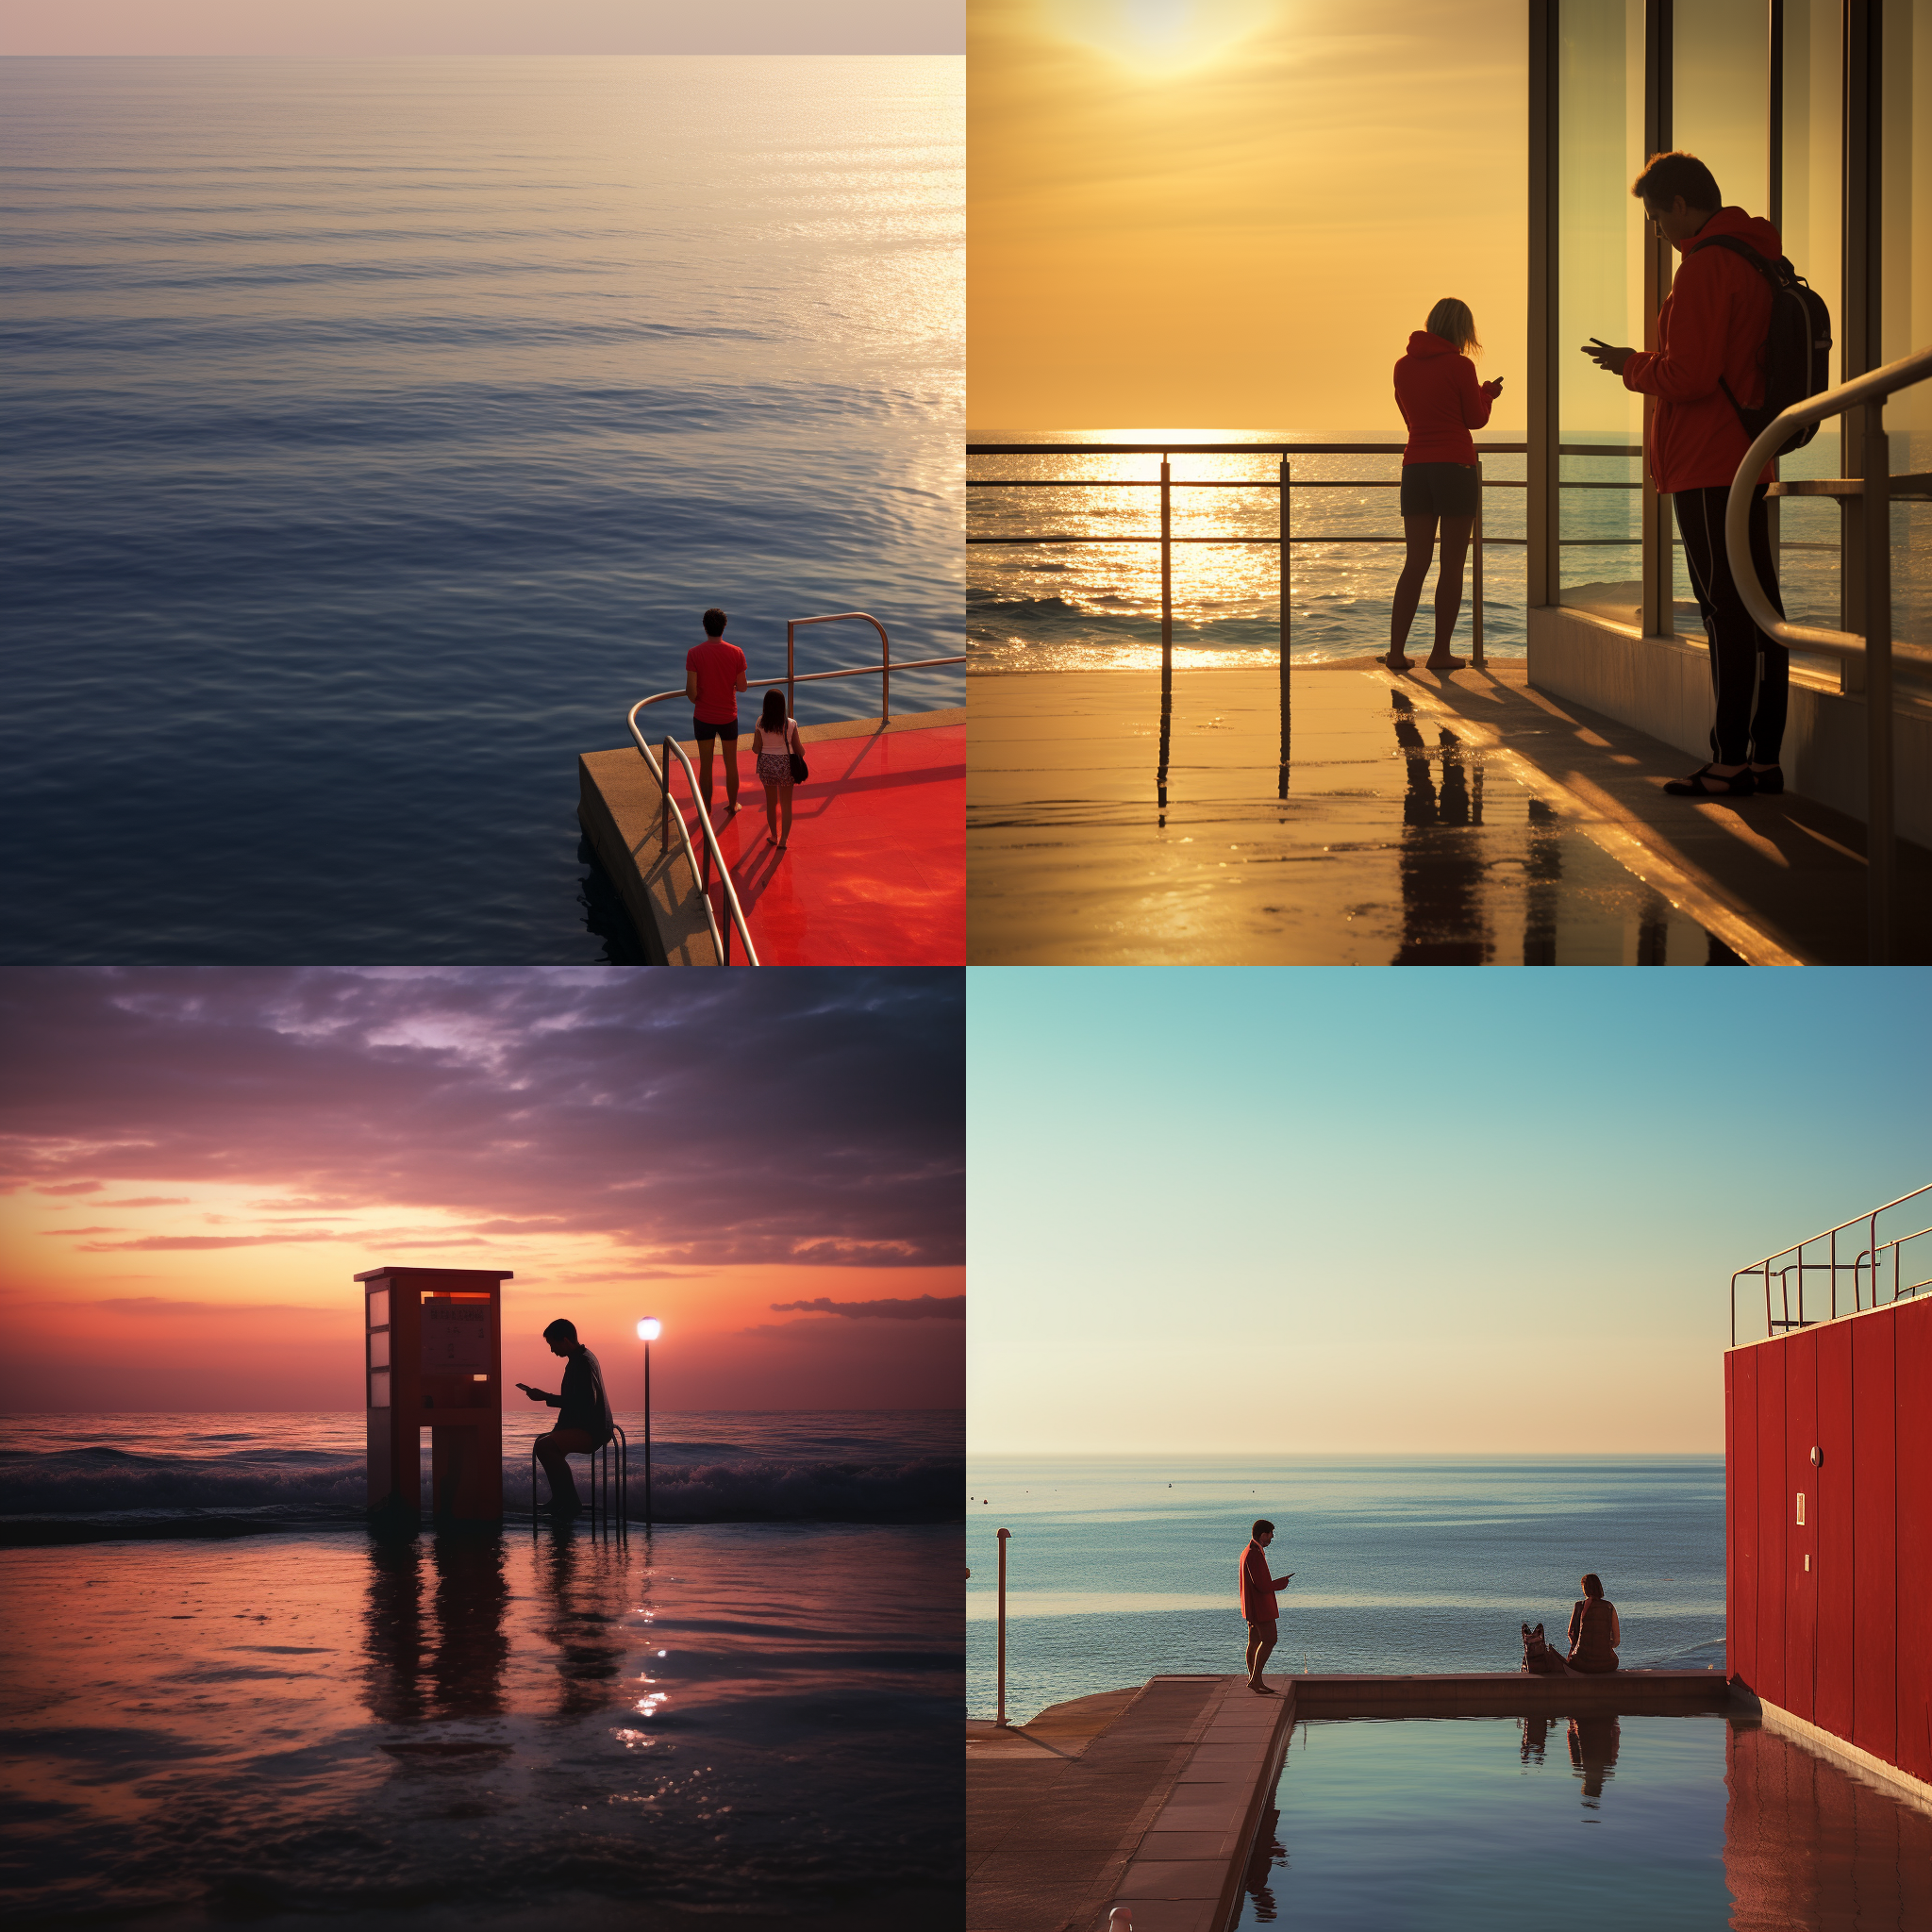
\includegraphics[width=0.5\textwidth]{midjourney_donfrodo_a_lifeguard_checking_his_iPhone_while_a_woman_is_drowning.png}
\caption{Generated via Midjourney by Donfrodo: A lifeguard checking his iPhone while a woman is drowning.}
\end{figure}


\tableofcontents

\newpage

\section{Introduction}

Imagine a person at sea is in trouble and another person on the beach or also in the water wants to save her.
The problem at hand involves finding the optimal path a person should take when transitioning from water to sand
or/and sand to water to reach the destination in the water in the shortest time possible.
Given the different speeds of the person on sand and water,
the problem can be approached mathematically to determine the best strategy.

\section{Sand to Water Case}

\subsection{Deriving the Route and its Total Time}

Given the scenario where a person transitions from sand to water, the total time taken can be derived based on the
distance covered on sand and water, as well as their respective speeds.

Let's assume the following:

\begin{align*}
x_1, y_1 & : \text{Coordinates of the starting point on sand} \\
x_2, y_2 & : \text{Coordinates of the target point in water} \\
x_3 & : \text{Horizontal coordinate where the person enters the water} \\
v_{sand} & : \text{Speed of the person on sand} \\
v_{water} & : \text{Speed of the person in water}
\end{align*}

The time taken for the sand portion is:

\[ T_{sand} = \frac{\sqrt{(x_3 - x_1)^2 + y_1^2}}{v_{sand}} \]

And for the water portion:

\[ T_{water} = \frac{\sqrt{(x_3 - x_2)^2 + (y_2 - 0)^2}}{v_{water}} \]

The total time is:

\[ T_{total} = T_{sand} + T_{water} \]


\subsection{Derivation of the Derivative and its Roots}

By differentiating \( T_{total} \) with respect to \( x_3 \) and setting the result to zero,
one can find the optimal value of \( x_3 \) that minimizes the total time.

Starting from:
\[ \frac{d T_{total}}{d x_3} = \frac{(x_3 - x_1)}{v_{sand} \cdot \sqrt{(x_3 - x_1)^2 + y_1^2}} - \frac{(x_3 - x_2)}{v_{water} \cdot \sqrt{(x_3 - x_2)^2 + y_2^2}} = 0 \]

Multiplying through by the common denominator gives:

\[ (x_3 - x_1) \cdot v_{water} \cdot \sqrt{(x_3 - x_2)^2 + y_2^2} = (x_3 - x_2) \cdot v_{sand} \cdot \sqrt{(x_3 - x_1)^2 + y_1^2} \]

Now, we'll square both sides to eliminate the square roots:

\[ (x_3 - x_1)^2 \cdot v_{water}^2 \cdot ((x_3 - x_2)^2 + y_2^2) = (x_3 - x_2)^2 \cdot v_{sand}^2 \cdot ((x_3 - x_1)^2 + y_1^2) \]


%Starting with the relationship:
%\[ (x_3 - x_1)^2 \cdot v_{water}^2 \cdot ((x_3 - x_2)^2 + y_2^2) = (x_3 - x_2)^2 \cdot v_{sand}^2 \cdot ((x_3 - x_1)^2 + y_1^2) \]

Expanding both sides and equating them:

\begin{align*}
& v_{water}^2 \cdot (x_3^4 - 2x_1x_3^3 + x_1^2x_3^2 + x_3^2x_2^2 - 2x_2x_3^3 + x_1^2x_2^2 + x_3^2y_2^2 - x_1^2y_2^2) \\
& = v_{sand}^2 \cdot (x_3^4 - 2x_2x_3^3 + x_2^2x_3^2 + x_3^2x_1^2 - 2x_1x_3^3 + x_1^2x_2^2 + x_3^2y_1^2 - x_2^2y_1^2)
\end{align*}

Grouping terms by their power of \(x_3\):

\begin{align*}
& x_3^4 \cdot (v_{water}^2 - v_{sand}^2) \\
& x_3^3 \cdot (2x_1v_{water}^2 + 2x_2v_{water}^2 - 2x_1v_{sand}^2 - 2x_2v_{sand}^2) \\
& x_3^2 \cdot (x_1^2v_{water}^2 + x_2^2v_{water}^2 + y_2^2v_{water}^2 - x_1^2v_{sand}^2 - x_2^2v_{sand}^2 - y_1^2v_{sand}^2) \\
& x_3 \cdot 0 \\
& \text{Constant} \cdot (x_1^2x_2^2v_{water}^2 - x_1^2y_2^2v_{water}^2 - x_1^2x_2^2v_{sand}^2 + x_2^2y_1^2v_{sand}^2)
\end{align*}

From the above grouping, the coefficients are derived as:

\begin{align*}
a & = v_{water}^2 - v_{sand}^2 \\
b & = 2x_1v_{water}^2 + 2x_2v_{water}^2 - 2x_1v_{sand}^2 - 2x_2v_{sand}^2 \\
c & = x_1^2v_{water}^2 + x_2^2v_{water}^2 + y_2^2v_{water}^2 - x_1^2v_{sand}^2 - x_2^2v_{sand}^2 - y_1^2v_{sand}^2 \\
d & = 0 \\
e & = x_1^2x_2^2v_{water}^2 - x_1^2y_2^2v_{water}^2 - x_1^2x_2^2v_{sand}^2 + x_2^2y_1^2v_{sand}^2
\end{align*}

Putting it all together, we have the \emph{quartic equation}\index{quartic equation}. in \( x_3 \):
\[ a \cdot x_3^4 + b \cdot x_3^3 + c \cdot x_3^2 + d \cdot x_3 + e = 0 \]

Given the complexity of quartic equations, finding its roots can be challenging,
especially if it doesn't factor conveniently.
Hence, we employ numerical methods to find the optimal value of \( x_3 \), as you will see in the python code below.

\subsection{Some Sand to Water Example Scenario's}

Figure \ref{fig:sand_to_water} displays some sand to water scenario's.

% The figure environment takes care of caption, positioning, etc.
\begin{figure}[htbp] % Positioning options: h=here, t=top, b=bottom, p=page, !=override
    \centering % Centers the image
    \includegraphics[width=1.0\textwidth]{sand_to_water.pdf} % The width parameter scales the image to 100% of the text width in this case
    \caption{Sand to Water Scenario's.} % Caption
    \label{fig:sand_to_water} % Reference label for cross-referencing
\end{figure}



\section{Water to Water Case}

\subsection{Deriving the Routes and their Total Time}

\subsubsection{Direct Swim Scenario}

Given the scenario where a person swims directly to the target point in the water, the time taken can be expressed as:

\[ T_{direct}(x_1, y_1, x_2, y_2, v_{water}) = \frac{\sqrt{(x_2 - x_1)^2 + (y_2 - y_1)^2}}{v_{water}} \]

Where \( x_1, y_1 \) are the coordinates of the starting point in water, \( x_2, y_2 \)
are the coordinates of the target point in water, and \( v_{water} \) is the speed of the person in water.
This time does not have to be optimised as it is not a function of any variable, rather a function of constants only.
However, its time value will be compared to the time taken of another route, as described in the next section.

\subsubsection{Swim to Coast, then Run, then Swim Scenario}

Given the scenario where a person first swims to the coast, runs on the sand, and then swims again to reach the
target point, the total time taken can be expressed as:

\begin{align*}
T_{combined}(x_1, y_1, x_2, y_2, x_3, x_4, v_{water}, v_{sand}) &= \frac{\sqrt{x_1^2 + y_1^2}}{v_{water}} + \frac{|x_3 - x_4|}{v_{sand}} \\
&+ \frac{\sqrt{(x_2 - x_4)^2 + y_2^2}}{v_{water}}
\end{align*}

Where:
\begin{itemize}
    \item \( x_1, y_1 \) are the coordinates of the starting point in water.
    \item \( x_2, y_2 \) are the coordinates of the target point in water.
    \item \( x_3 \) is the horizontal coordinate where the person exits the water onto the coast.
    \item \( x_4 \) is the horizontal coordinate where the person enters the water again after running on the sand.
    \item \( v_{sand} \) is the speed of the person on sand.
    \item \( v_{water} \) is the speed of the person in water.
\end{itemize}

The optimization problem aims to find the values of \( x_3 \) and \( x_4 \) (where the person enters the water again)
that minimize \( T_{combined} \). This problem can't be easily solved symbolically, necessitating the use of
\emph{multivariable optimization}\index{multivariable optimization} techniques. This can be seen in the python code below.

\subsection{Some Water to Water Example Scenario's}

Figure \ref{fig:water_to_water} displays some water to water scenario's.

% The figure environment takes care of caption, positioning, etc.
\begin{figure}[htbp] % Positioning options: h=here, t=top, b=bottom, p=page, !=override
    \centering % Centers the image
    \includegraphics[width=1.0\textwidth]{water_to_water.pdf} % The width parameter scales the image to 100% of the text width in this case
    \caption{Water to Water Scenario's.} % Caption
    \label{fig:water_to_water} % Reference label for cross-referencing
\end{figure}


\section{Python Code}

The following python code implements all scenario's and also produces the figures
\ref{fig:sand_to_water} and \ref{fig:water_to_water} as output pdfs.

\lstinputlisting[language=Python, caption=BeachBiz26.py]{BeachBiz26.py}

\printindex

\end{document}

